\documentclass{beamer}
\usetheme{metropolis}
\usepackage[font=footnotesize, labelfont=footnotesize]{caption}



\title{Future of Web Development Technology}
\subtitle{Demo teaching}
\date{16 November 2016}
\author{Steven "Steven"}
\institute{BINUS INTERNATIONAL}


\begin{document}
  \maketitle
  
%  \section {Class organization}
  \begin{frame}{Some basic rules}
  	\begin{itemize}
%		\item Phone should be silent at all time
%		\item Laptop is okay
		\item Questions, for this specific session, should be put on hold until the end of presentation
		\item All slides and materials are available at github (goo.gl/Lb2VQQ) (Corrections to them are encouraged)
	\end{itemize}
  \end{frame}
  
  \begin{frame}{Quick introduction}
	Steven "Steven"
	
	Graduated from The University of Edinburgh (2016), Binus International (2012)
	
	Professionally worked on:
	\begin{itemize}
		\item stamps.co.id  (Everything)
		\item go-jek.com (iOS alpha)
		\item setipe.com  (iOS)
		\item anomalicoffee.com (iOS, Web backend)
		\item fotostruk.com (Upcoming)
	\end{itemize}
	
	Github profile: https://github.com/SeiryuZ
  \end{frame}
  
    \begin{frame}{Web development?}
	Anything related to developing a web site for the internet or intranet.
	
	\pause
	Typically, web development is divided into two:
	
	\pause
	\begin{itemize}[<+->]
		\item \textbf{Back-end}, Development of application on the server-side that accept requests from the user, and produce the correct output (Python, Ruby, Java, ........)  
		
		\item \textbf{Front-end}, Development of client-side application that allows user to interact with the web-site directly. (CSS, HTML, JS)
		
		\item Think of Back-end as house builder and Front-end as Interior design when you build a house
	\end{itemize}
    \end{frame}

  
%  \section{Motivation}
  \begin{frame}{Why web development?}
	\pause
	Q: We can develop application for users' device "easily", why bother with web development?

	\pause
	\begin{itemize}[<+->]
	
		\item Internet user is almost half of Earth's population (3,4b/46\% as of 1 June 2016)\footnotemark[1]
			\begin{itemize}[<+->]
				\item around 20\% of Indonesia population are connected to Internet (50m in 2016\footnotemark[1])
			\end{itemize}
			
		\item Arguably, web have smaller permutation of end-user run time environments (Web browser, Web Client).
		
		\item Offloading computations to much powerful, and potentially infinite resources (Cloud computing)
		
		\item Huge number of open source software that can be used for your project
		
	\end{itemize}
	\only<2->{\footnotetext[1]{http://www.internetlivestats.com/internet-users/}}

  \end{frame}
  
  
  
  \begin{frame}{That's all good, there has to be some downside, right?}
  	\pause
	Backend:
	\pause
	\begin{itemize}[<+->]
		\item Backend: Deploying web application
		\item Future of Backend ? \pause Containerization (Docker / LXC)
  	\end{itemize}
  \end{frame}
  
    \begin{frame}{That's all good, there has to be some downside, right?}
  	\pause
	Frontend
	\pause
	\begin{itemize}[<+->]
		\item Frontend: Web development standard
		\item Future of frontend ? \pause Sane web standard (js.foundation)
  	\end{itemize}
	\pause
	\begin{center}
		\begin{figure}
		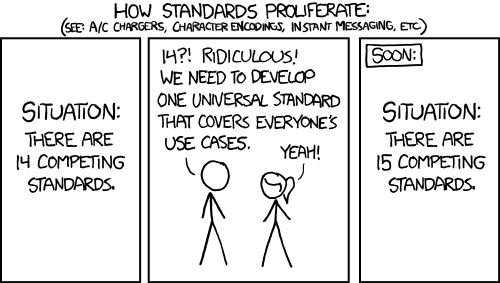
\includegraphics[scale=0.485]{images/standards.png}
		\caption{xkcd.com}
		\end{figure}
	\end{center}
  \end{frame}
  
  
%   \begin{frame}{Future of Web Development Technology}
%   	\pause
%	\begin{itemize}[<+->]
%		\item Backend: Containerization / Virtualization (Docker, Linux Containers)
%		\item Frontend: Better web standard \footnotemark[1] \footnotemark[2] 
%	\end{itemize}
%	\pause
%	\begin{center}
%		\begin{figure}
%		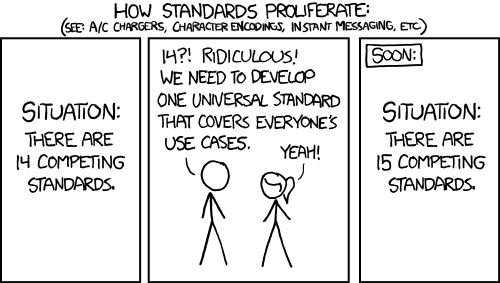
\includegraphics[scale=0.485]{images/standards.png}
%		\caption{xkcd.com}
%		\end{figure}
%	\end{center}
%
%	\only<3->{\footnotetext[1]{See http://caniuse.com}}
%	\only<3->{\footnotetext[2]{See https://js.foundation}}
%  \end{frame}
%%  
%  \begin{frame}{Future of Web Development Technology - Containerization}
%	Complex backend development requires huge number of inter-dependent technologies to run correctly. For example, database system, application server, file server, web server, cache service, data structure service and queue systems. 
%	
%	More concrete, stamps.co.id backend requires more than 50 libraries and technologies to run correctly. All of these libraries needs to be configured correctly for the web service to run. 
%	
%	In addition to that, correctly configuring all of these for multiple servers (Usually, web services have multiple hosts containing different services) are time consuming and error-prone, even with some automation.
%	
%	Containerization aims to solve this by allowing developers to package everything inside a containers. And target hosts, your server, only need to be able to run your containers. These abstractions would allow development and deployment with ease.
%	
%  \end{frame}
%  
%  \begin{frame}{Future of Web Development Technology - Web development standard}
%	JS Foundation, under The Linux Foundation, are pushing a new set of standards for web development, specifically on the Javascript ecosystem. The foundation is "blessing" some of the most important projects that  open web development relies on. 
%	
%	This move hopes to settle the debate on what tools to use, and help the community get organized in contributing towards the "blessed" projects. In the future, front-end web development might have better tools and universally agreed standards to make it easier to do development.
%  \end{frame}
%  
  
  %% IOT Slide??
\end{document}